% Description of what testing you did and any test frameworks that were usedi
\section{Performance Tests and Analysis}
\label{Performance Tests and Analysis}

Timing and profiling runs were performed on the CP Lab machines due to the availability of a working version of gprof, which was not present on all of the group's own computers.
Optimisation was performed in two stages: changes to the code, and changes to the compiler optimisation flags.  For the first stage the \texttt{-O3} flag was used for all runs.  The second stage chose the best-performing version of the program from the first stage and observed the effects of compiling with the \texttt{-O4} and \texttt{-O5} flags.
Run time of the program was measured over a series of square landscapes with sizes ranging from 200x200 to 2000x2000.
Profiling runs were performed using an 800x800 landscape.
All timing runs were configured to perform 1250 time steps with PPM file output every 100 time steps.


\subsection{Code optimisation}
\label{Code optimisation}

\begin{table}[h!]
\caption{Tabulated partial output from gprof on first profiled version of popsim.}
\label{tab:profile1}
\begin{center}
\begin{tabular}{|c|c|c|c|c|}
\hline
time [\%] & time [s] & self time [s] & calls & name\\
\hline
47.00 & 58.77 & 58.77 & 1250 & $Landscape::Update()$\\
\hline
24.30 & 89.15 & 30.38& 4806406416 & $Array2D::operator()$\\
\hline
10.75& 102.59 & 13.44 & 511439120 & $std::vector::operator[]$\\
\hline
\end{tabular}
\end{center}
\end{table}

Table \ref{tab:profile1} shows partial output from gprof for the initial version of the code.
Three functions accounted for approximately 82\% of the run time, with nearly half of the run time spent in \texttt{Landscape::Update()}.
This was to be expected as the bulk of the program's work was done in this function.
However there were six orders of magnitude more calls to Array2D::operator() than to \texttt{Landscape::Update()} consuming nearly one quarter of the run time.  This suggested a simple modification: removing the bounds checking on every element access in \texttt{Array2D<T>::operator()}.
This change was made and a second timing run and profiling run were done.

\begin{table}[h!]
\caption{Tabulated partial output from gprof after array bounds checking removal.}
\label{tab:profile2}
\begin{center}
\begin{tabular}{|c|c|c|c|c|}
\hline
time [\%] & time [s] & sef time [s] & calls & name\\
\hline
50.30 & 58.25 & 58.25 & 1250 & $Landscape::Update()$\\
\hline
15.18 & 75.83 & 17.58 & 4806406416 & $Array2D::operator()$\\
\hline
13.72 & 91.71 & 15.89 & 511439120 & $std::vector::operator[]$\\
\hline
\end{tabular}
\end{center}
\end{table}

Table \ref{tab:profile2} shows partial output from gprof for the version of the code with array bounds removed.
The time spent in \texttt{Array2D::operator()} was significantly reduced compared to the first profiling run.
While bounds checking was included in the initial version of \texttt{Array2D<T>::operator()} for safety, once the program had been demonstrated to work correctly, the considerable performance improvement achieved by removing bounds checking was considered to be worthwhile.

The group later learned from the reference documentation for class \texttt{std::vector} that element access with bounds checking is provided by the function \texttt{std::vector<T>::at()}.
However, it was assumed that even bounds checking performed by the standard library which is typically very well optimised would be slower than no bounds checking at all.
Code for all three options was left in the code in \texttt{Array2D::operator()()} with the unused options commented out.

A second optimisation became apparent on examination of the for loops in \texttt{Landscape::Update()}.
The code was iterating over the x-coordinate of a cell, then over its y-coordinate.
While this was the intuitive order, it caused the code to stride through the array of cells by a distance proportional to the width of the landscape array instead of accessing the next cell in memory each time.
The order of the iterations was swapped, and another profiling and timing run were performed.

\begin{table}[h!]
\caption{Tabulated partial output from gprof after iteration order swap.}
\label{tab: profile 3}
 \begin{center}
\begin{tabular}{|c|c|c|c|c|}
\hline
name & time [\%] & time [s] & sef time [s] & calls\\
\hline
$Landscape::Update()$ & 48.54 & 59.65 & 59.65 &1250 \\
\hline
$Array2D::operator()$& 17.45& 81.10& 21.45 &4806406416 \\
\hline
$std::vector::operator[]$& 12.34& 96.27 &15.17 &511439120\\
\hline
\end{tabular}
\end{center}
\end{table}

Table \ref{tab: profile 3} shows partial output from gprof for the version of the code with array bounds removed and with iteration order reversed.
This version spent a slightly lower percentage of its run time in function \texttt{Landscape::Update()}.
The improvement in performance was less than expected given that memory loading into cache was theoretically optimised. Fig.(\ref{fig:Optimisation}) shows the timing for the different optimisation steps.

\begin{figure}
\begin{center}
  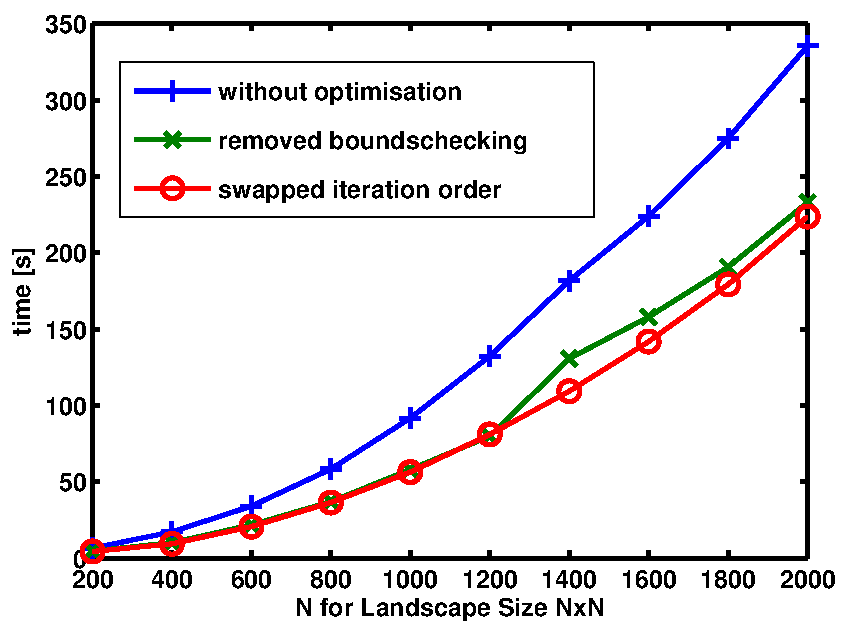
\includegraphics[scale=0.7]{Figures/TimingsOptimisation.pdf}
\caption{A comparison of timings for the different optimasation stages.}
\label{fig:Optimisation}
\end{center}
\end{figure}


A further optimisation was considered but not implemented due to time constraints: storing pointers to cell neighbours in each cell so that function \texttt{Landscape::Update()} could access each cell's neighbours without calling \texttt{Array2D::operator()} four times.
These pointers would be initialised at program startup meaning the array accesses would be done just once instead of once per update and reducing the number of memory accesses to non-local parts of the array.
However, there was insufficient time for this change to be implemented and tested.\\

The group also considered checking whether any difference in performance could be found between runs on landscapes with different arrangements of land and water due to branch prediction as the Landscape class verifies that cell is land before performing the calculation for that cell.
A landscape consisting entirely of islands of one cell would presumably cause the branch prediction to be wrong most if not all of the time, which would presumably reduce performance compared to a landscape with the same number of land cells arranged at the top or bottom of the landscape, corresponding to the beginning or end of the landscape array.


\subsection{Compiler optimisation.}
\label{Compiler optimisation}

To compare program timings we define the pogram speedup as

\begin{equation}
S = 1-T/ T_{ref}
\label{equation:speedup}
\end{equation}

where $T_{ref}$ is the time taken by an initial reference run and ${T}$ is the time taken by a run for which the speedup is being calculated. This provides an adequate messure since it is positive if the new run is faster than the reference run and vice versa. 

Fig.(\ref{fig: Comp flags bahart}) shows a comparison of builds with different compiler optimisation flags \texttt{-O4}/\texttt{-O5} with reference to the \texttt{-O3} optimised version using the speed up defined in eq.(\ref{equation:speedup}).

\begin{figure}
\begin{center}
 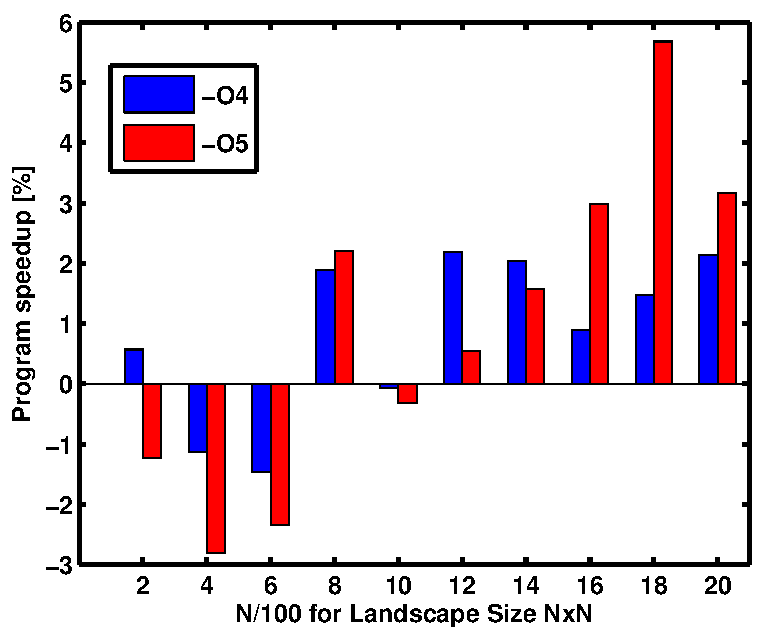
\includegraphics[scale=0.8]{Figures/Timing_Barchart_compflags.pdf}
\caption{The effect of compiler flags in percentage of the \texttt{-O3} timings.}
\label{fig: Comp flags bahart}
\end{center}
\end{figure}

It was found that the various compiler optimisation flags made only a slight improvement for some landscape sizes and actually reduced performance in some cases.


\subsection{Scaling perfomance}
\label{subsec:scaling pefomance}

To investigate the progamms performance, its time scaling with increased landscape size was investigated.
To this end, the timing data, with the compiler flag  \texttt{-O5}, was fitted to the expected quadratic behaviour

\begin{equation}
 T(N)=a+bN^2
\label{eq:fitting curve}
\end{equation}

where a constant term $a$ was included to substract a possibly unifom system overhead common to all sizes.
The fit was performed with a nonlinear regression model using least squares, yielding the optimal parameters $a=2.36 [s]$ and $b=5.29*10^{-6} [s/N^2]$.
As can be seen from fig.(\ref{fig:fitting curve}) the fit matches very well to the data points which is confirmed by an R-squared value $R=0.999$ characterising the fit.
This suggests that the pogram's perfomance scales quadratically as is to be expected for a problem defined on a two dimensional grid.

\begin{figure}
 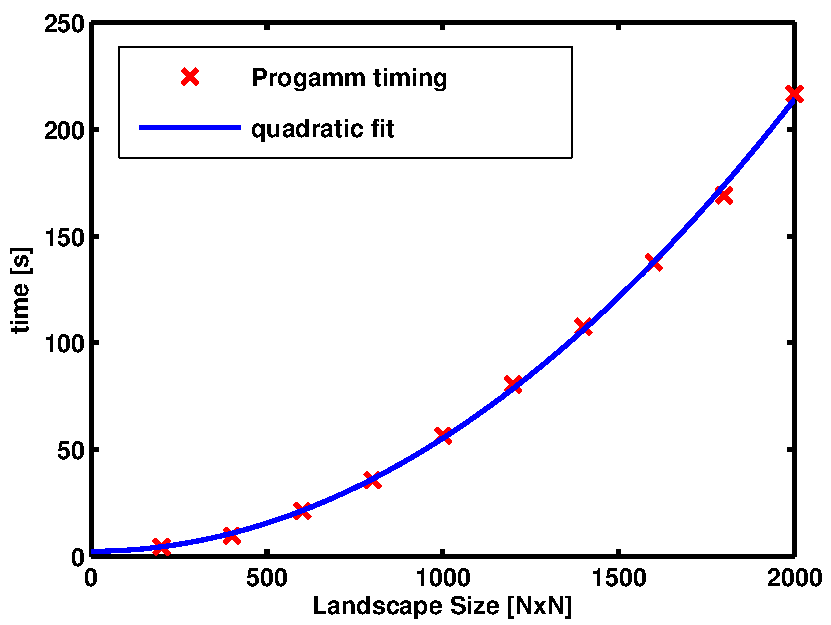
\includegraphics{Figures/TimingFitO5.pdf}
\caption{A quadratic fit, see eq.(\ref{eq:fitting curve}), for the program perfomance.}
\label{fig:fitting curve}
\end{figure}








